\chapter{Resultados Parciais: Primeira contribui\c{c}\~ao}

\section{Feixes Escalares puramente propagantes com simetria azimutal}
Com o objetivo de validar a metodologia proposta, foram estudados tr\^es tipos de espectros: exponencial, gaussiano e quadrado. Os resultados obtidos foram feitos no software $Matlab$. Consideramos o v\'acuo ($c=3.10^8 m/s$) e o comprimento de onda $\lambda = 0,632.10^{-6}m$ (isto \'e, com $\omega = 2,98.10^{15}Hz$). 
%************************************************************************************************************************
\subsection{Espectro exponencial} O espectro exponencial foi definido por:
\begin{equation}\label{e1}
S(k_{z})= \left\{
\begin{array}{rcl}
   \frac{1}{K}\exp[-a(\omega /c - k_z )];  & , & 0\leq k_{z}\leq \omega /c\\
     0 &  , & $caso contr\'ario$
\end{array}
\right.
\end{equation}
onde $K=2\omega/c$. A largura de banda $\Delta k_z$ do espectro \'e diretamente proporcional ao valor de $1/a$, o qual determina se o espectro exponencial \'e do tipo paraxial ou n\~ao paraxial. Nesse caso a solu\c{c}\~ao sai diretamente, sem a necesidade de expandir $S(k_z)$ em s\'eries de Fourier.\\
Substituindo (\ref{e1}) na solu\c{c}\~ao (\ref{eqA4}) temos:
\begin{equation}\label{z2}
    \psi(\rho,z,t)= \frac{c}{2\omega}\exp[-{\rm i}\omega t]\int_{-\omega/c}^{\omega/c}J_0(\rho\sqrt{\omega^2/c^2-k_{z}^2})\exp[{\rm i}k_{z}z]\exp[-a(\omega/c-k_{z})]d k_{z}
\end{equation}
Seja $k_{z}=(\omega/c)s$, ent\~ao $d\kappa_{z}=(\omega/c)ds$. Substituindo em (\ref{z2}):
\begin{eqnarray}
\psi(\rho,z,t) &=&\frac{c}{2\omega}\exp[-{\rm i}\omega t]\int_{-1}^{1}J_0(\rho\sqrt{\frac{\omega^2}{c^2}-\frac{\omega^2}{c^2}s^2})\exp[{\rm i}\frac{\omega}{c}s z]\exp[-a(\omega/c-\omega s/c)]\frac{\omega}{c}ds\nonumber\\
 &=&\frac{c}{2\omega} \frac{\omega}{c}\exp[-{\rm i}\omega t-a\omega/c]\int_{-1}^{1}J_0(\frac{\omega}{c}\rho\sqrt{1-s^2})\exp[{\rm i}(z-{\rm i}a)\frac{\omega}{c}s]ds
\label{z3}
\end{eqnarray}
expandendo o termino $\exp[{\rm i}(z-{\rm i}a)\frac{\omega}{c}s]$ na forma trigonom\'etrica, temos:
\begin{equation}\label{z4}
   \psi(\rho,z,t)=\exp[-{\rm i}\omega t-a\omega/c]sinc[\sqrt{\frac{\omega^2}{c^2}\rho^2+\frac{\omega^2}{c^2}(z-{\rm i}a)^2}]
\end{equation}
Reparar que os feixes dados em ($\ref{z4}$) s\~ao solu\c{c}\~oes ana\'iticas exatas da equa\c{c}\~ao de onda, onde n\~ao surgiu a necessidade de obter as solu\c{c}\~oes mediante os coeficientes de Fouries dados em (\ref{eqA20}) com (\ref{eqA19}).\\
%*******************************************************************************
%*******************************************************************************
\begin{figure}[h]
\centering
\subfigure[]{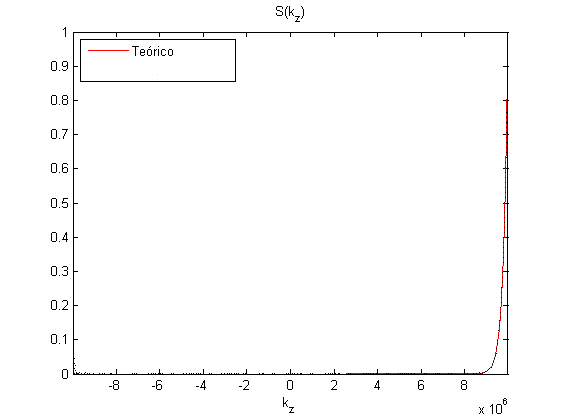
\includegraphics[scale=0.3]{figex1a.png}}
\centering
\subfigure[]{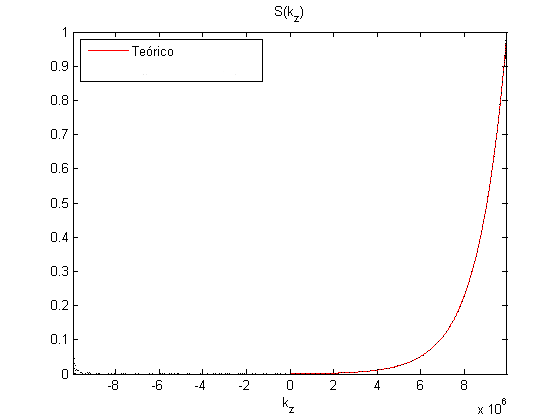
\includegraphics[scale=0.3]{figex2a.png}}\\
\centering
\subfigure[]{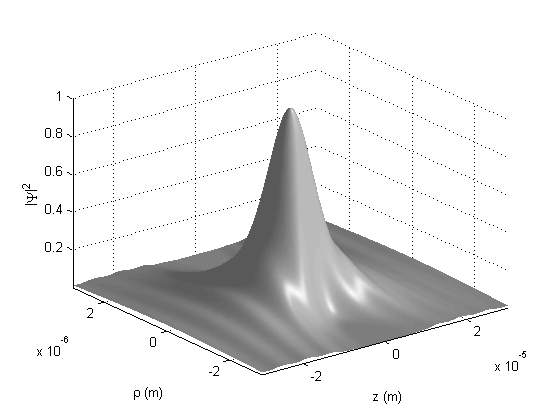
\includegraphics[scale=0.3]{figex1b.png}}
\centering
\subfigure[]{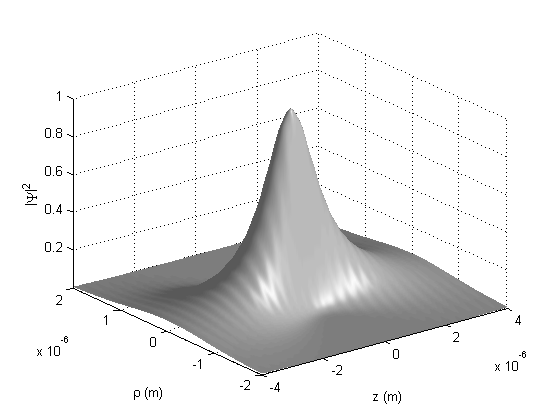
\includegraphics[scale=0.3]{figex2b.png}}\\
\centering
\subfigure[]{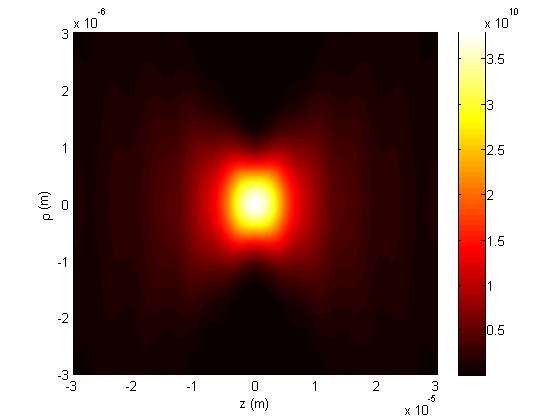
\includegraphics[scale=0.3]{figex1c.png}}
\centering
\subfigure[]{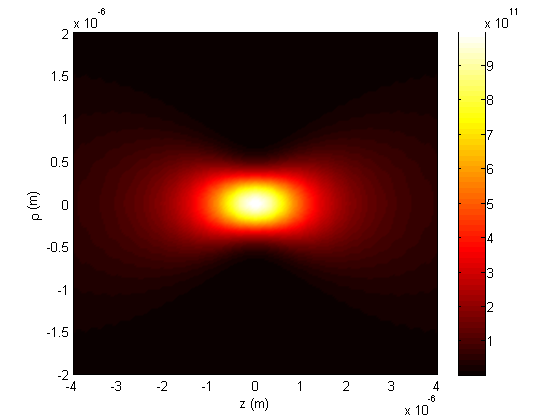
\includegraphics[scale=0.3]{figex2c.png}}\\
\caption{(a)-(b) Gr\'aficos do espectro exponencial paraxial e n\~ao paraxial respectivamente. Os tra\c{c}os em vermelhos representam o espectro dado pela eq. (\ref{e1}). (c)-(d) Padr\~oes de intensidade 3D, solu\c{c}\~oes exatas da equa\c{c}\~ao de onda dos feixes paraxial e n\~ao paraxial respectivamente dados pela eq. (\ref{z4}). (e)-(f) Proje\c{c}\~ao ortogonal da intensidade do feixe exponencial no plano $(\rho,z)$.}
\label{fig1}
\end{figure}
%*******************************************************************************
%*******************************************************************************
Foram analisados dois tipos de espectros: O primeiro, um espectro do tipo paraxial para gerar feixes paraxiais.\\
 Para obter um feixe paraxial, nosso espectro $S(k_z)$ foi concentrado ao redor de $\bar{k}_z = \omega /c=9,97.10^6 m^{-1}$, com $\Delta k_z =1/a = K/100  = 0,199.10^6 m^{-1}\ll \omega /c$ e onde $\Delta k_z/\bar{k}_z=0,02\ll 1$. O gr\'afico te\'orico do espectro paraxial (\ref{e1}) \'e mostrado na Figura \ref{fig1}(a) em cor vermelha.\\
O segundo espectro foi do tipo n\~ao paraxial, com uma largura de banda maior que a primeira $\Delta k_z = 1/a = K/20 = 0,997.10^6 m^{-1}$ e com $\Delta k_z/\bar{k}_z= 0,1$. O gr\'afico do espectro (\ref{e1}) desse segundo caso \'e mostrado na Figura \ref{fig1}(b) em cor vermelha.
Nas figuras \ref{fig1}(c)(d) s\~ao apresentados os padr\~oes de intensidade normalizados em 3D. A Figura \ref{fig1}(c) corresponde ao espectro paraxial obtido da Figura \ref{fig1}(a) e a Figura \ref{fig1}(d) corresponde ao espectro n\~ao paraxial obtido da Figura \ref{fig1}(b). Os feixes obtidos prov\^em de espectros n\~ao paraxiais e paraxiais e s\~ao solu\c{c}\~oes anal\'iticas exatas da equa\c{c}\~ao de onda.\\
Nas Figuras \ref{fig1}(e)(f) s\~ao apresentadas as proje\c{c}\~oes ortogonais das intensidades dos feixes \ref{fig1}(c)(d) no plano $(\rho,z)$. Podemos observar que os feixes produzidos s\~ao propagantes e possuem simetria azimutal.
%*************************************************************************************************************************
\subsection{Espectro quadrado} Seja um espectro quadrado definido por:
\begin{equation}\label{q1}
S(k_{z})= \left\{
\begin{array}{rcl}
     K= 2\omega/c & , & k_{zmin}\leq k_{z}\leq k_{zmax}\\
     0 &  , & $caso contr\'ario$
\end{array}
\right.
\end{equation}
onde $0\leq k_{zmin}\leq k_{zmax}  \leq\omega/c$. A posi\c{c}\~ao do espectro $\bar{k}_z$ e a largura de banda $\Delta k_z=k_{zmax}-k_{zmin}$, determinar\~ao se o espectro quadrado \'e do tipo paraxial ou n\~ao paraxial.\\
Substituindo (\ref{q1}) em (\ref{eqA19}), foram obtidos os coeficientes de Fourier $R_n$ do espectro quadrado $S(k_z)$. Para achar as solu\c{c}\~oes anal\'iticas exatas correspondentes ao espectro quadrado foram substitu\'idos os valores de $R_n$ em (\ref{eqA20}).\\
%*******************************************************************************
%*******************************************************************************
\begin{figure}[h]
\centering
\subfigure[]{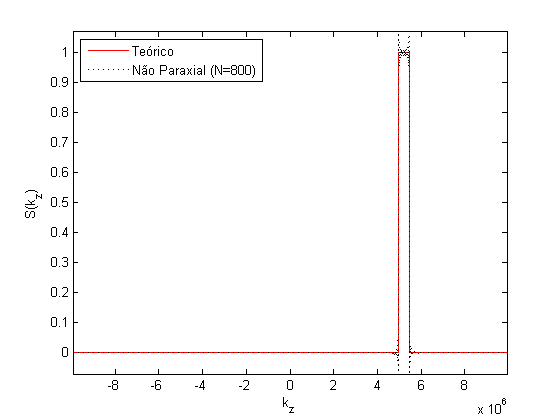
\includegraphics[scale=0.3]{figqu1a.png}}
\centering
\subfigure[]{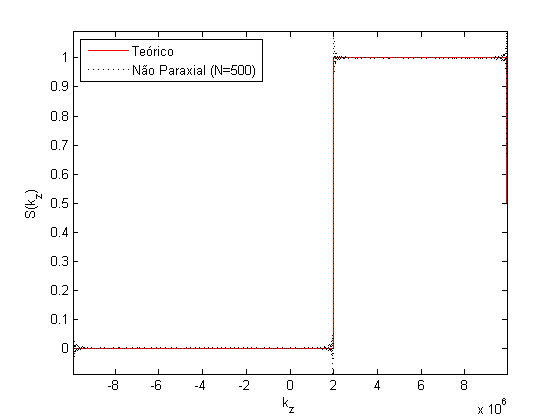
\includegraphics[scale=0.3]{figqu2a.png}}\\
\centering
\subfigure[]{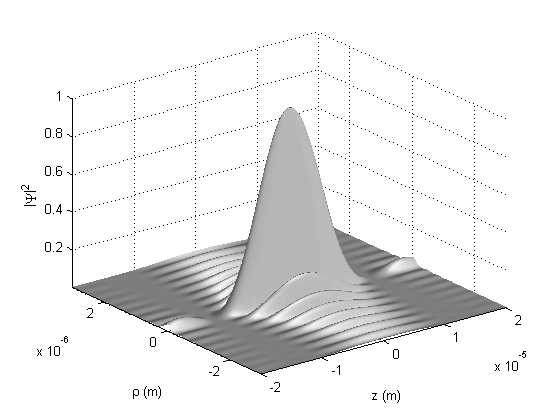
\includegraphics[scale=0.3]{figqu1b.png}}
\centering
\subfigure[]{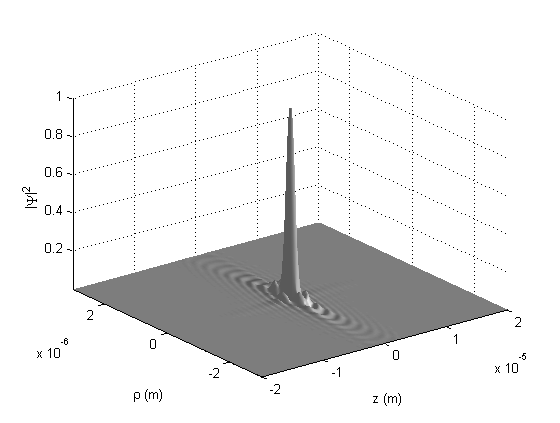
\includegraphics[scale=0.3]{figqu2b.png}}\\
\centering
\subfigure[]{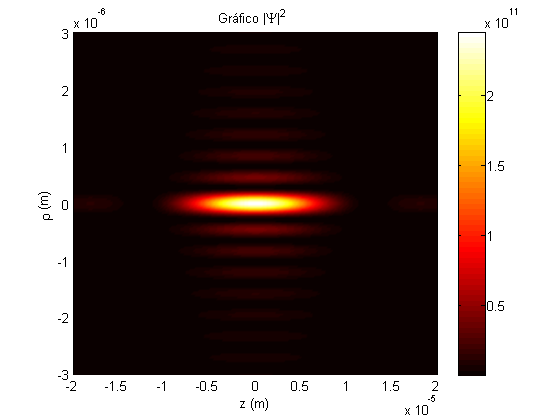
\includegraphics[scale=0.3]{figqu1c.png}}
\centering
\subfigure[]{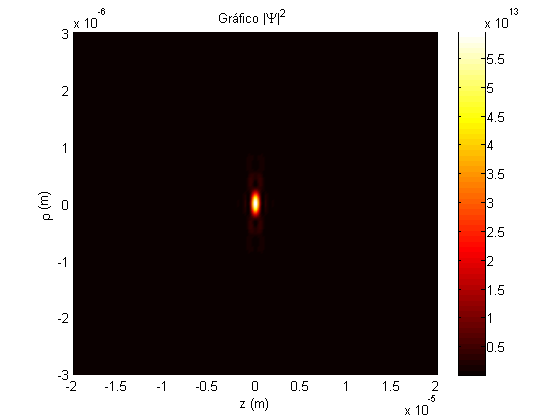
\includegraphics[scale=0.3]{figqu2c.png}}\\
\caption{(a)-(b) Gr\'aficos do espectro quadrado n\~ao paraxial. Os tra\c{c}os em vermelhos representam o espectro dado pela eq. (\ref{q1}). Os tra\c{c}os em cor preta representam a representa\c{c}\~ao de (\ref{q1}) atrav\'es da s\'erie de Fourier dada por (\ref{eqA19}). O n\'umero de termos de coeficientes de Fourier, para os  gr\'aficos foi de 1601 e 1001 respectivamente. (c)-(d) Padr\~oes de intensidade 3D, solu\c{c}\~oes exatas da equa\c{c}\~ao de onda dos feixes n\~ao paraxiais. (e)-(f) Proje\c{c}\~ao ortogonal da intensidade do feixe quadrado no plano $(\rho,z)$.}
\label{fig2}
\end{figure}
%*******************************************************************************
%*******************************************************************************
Foram analisados dois tipos de espectros n\~ao paraxiais.\\
O primeiro, um espectro concentrado em $\bar{k}_z=5,24.10^{6}m^{-1}$ com largura de banda de $\Delta k_z= 4,99.10^{5}m^{-1}$, com $k_{zmin}=4,99.10^{6}m^{-1}$ e $k_{zmax}=5,49.10^{6}m^{-1}$ e com $\Delta k_z/\bar{k}_z=0,095$. O gr\'afico do espectro (\ref{q1}), no primeiro caso, \'e mostrado na Figura \ref{fig2}(a) em cor vermelha, sendo a sua representa\c{c}\~ao atrav\'es da s\'erie de Fourier (\ref{eqA18}) e mostrada em cor preta. O n\'umero total de coeficientes de Fourier usado foi de $1601$, ou seja $N=800$.\\
O segundo espectro foi para uma largura de banda maior que a primeira $\Delta k_z= 7,98.10^{6}m^{-1}$ concentrado em $\bar{k}_z=5,99.10^{6}m^{-1} $, com $k_{zmin}=1,99.10^{6}m^{-1}$ e $k_{zmax}=9,98.10^{6}m^{-1}$, e com $\Delta k_z/\bar{k}_z=1,332$. O gr\'afico do espectro (\ref{q1}) desse segundo caso \'e mostrado na Figura \ref{fig2}(b) em cor vermelha, sendo a sua representa\c{c}\~ao atrav\'es da s\'erie de Fourier (\ref{eqA18}) \'e mostrada em cor preta. O n\'umero total de coeficientes de Fourier usado para este \'ultimo espectro foi de $1001$, ou seja $N=500$.\\
Na Figura \ref{fig2}(c)-(d) s\~ao apresentados os padr\~oes de intensidade em 3D. A Figura \ref{fig2}(c) corresponde ao espectro n\~ao paraxial obtido da Figura \ref{fig2}(a) e a Figura \ref{fig2}(d) corresponde a um espectro menos concentrado, obtido da Figura \ref{fig2}(b). Pode-se observar que o espectro mais concentrado (Figura \ref{fig2}(a)) produz uma maior propaga\c{c}\~ao do feixe. Os feixes produzidos possuem simetria azimutal.\\
Na Figura \ref{fig2}(e)-(f) s\~ao apresentadas as proje\c{c}\~oes ortogonais das intensidades dos feixes no plano $(\rho,z)$.  Os feixes obtidos prov\^em de espetros n\~ao paraxiais e s\~ao solu\c{c}\~oes anal\'iticas exatas da equa\c{c}\~ao de onda.\\
Para um espectro com largura de banda de $\Delta k_z=4,99.10^{6}m^{-1}$, o feixe n\~ao paraxial tem um spot com raio inicial igual a $0,4.10^6m$ aproximadamnete e uma profundidade de campo de $10,0.10^{-6}$m (Figura $\ref{fig2}$(e)). Para um espectro com largura de banda maior de $\Delta k_z=7,98.10^{6}m^{-1}$ , o raio do spot \'e de tamb\'em de $0,4.10^6m$ e a profundidade do campo do feixe n\~ao paraxial \'e de $0,1.10^{-5}$m (Figura $\ref{fig2}$(f)). Portanto, o feixe com espectro mais concentrado (Figura \ref{fig2}(a)), menor largura de banda, possui uma profundidade maior em rela\c{c}\~ao ao feixe menos concentrado (Figura \ref{fig2}(b)). Repare tamb\'em que os raios dos spots dos feixes produzidos s\~ao do ordem do comprimento de onda ($\lambda = 0,632.10^6m$), o qual caracteriza um feixe n\~ao paraxial.  
%**************************************************************************************************************************
\subsection{Espectro gaussiano} Seja um espectro gaussiano definido por:
\begin{equation}\label{ga1}
S(k_{z})= \left\{
\begin{array}{rcl}
  2(\omega/c)\exp(-a(k_z - \bar{k}_z)^2) & , & 0\leq k_{z}\leq \omega/c\\
     0 &  , & $caso contr\'ario$
\end{array}
\right.
\end{equation}
Onde $\bar{k}_z$ indica a posi\c{c}\~ao do centro do espectro. A largura de banda $\Delta k_z$ do espectro \'e diretamente proporcional ao valor do desvio padr\~ao $1/\sqrt{(2a)}$, o qual determina se o espectro gaussiano\'e do tipo paraxial ou n\~ao paraxial.  \\
Substituindo (\ref{ga1}) em (\ref{eqA19}), foram obtidos os coeficientes de Fourier $R_n$ do espectro gaussiano $S(k_z)$. Para obter as solu\c{c}\~oes anal\'iticas exatas correspondentes ao espectro gaussiano foram substitu\'idos os valores de $R_n$ em (\ref{eqA20}).\\
%*******************************************************************************
%*******************************************************************************
\begin{figure}[h]
\centering
\subfigure[]{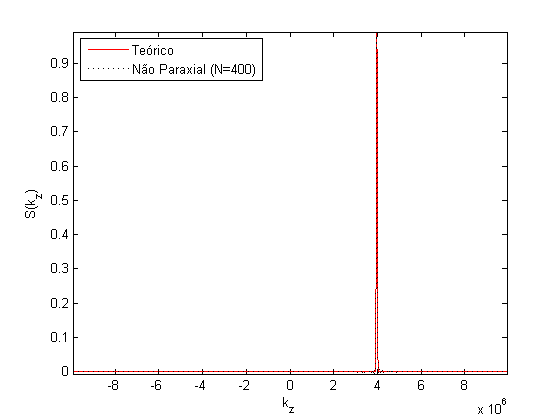
\includegraphics[scale=0.3]{figgau1a.png}}
\centering
\subfigure[]{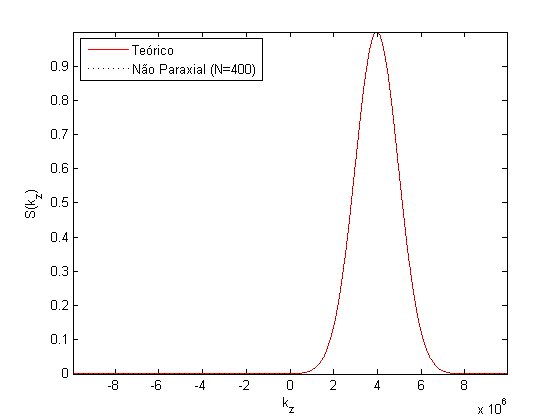
\includegraphics[scale=0.3]{figgau2a.png}}\\
\centering
\subfigure[]{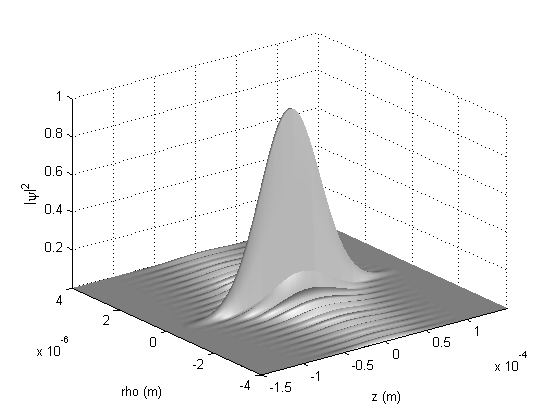
\includegraphics[scale=0.3]{figgau1b.png}}
\centering
\subfigure[]{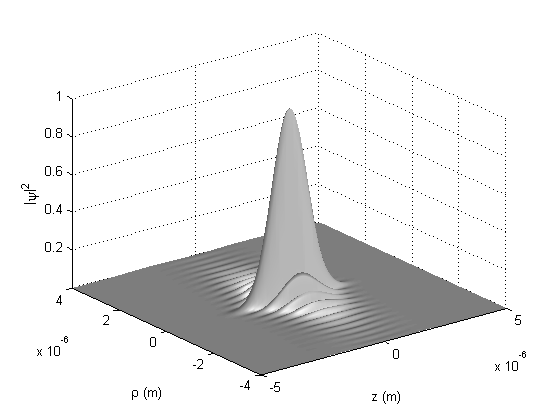
\includegraphics[scale=0.3]{figgau2b.png}}\\
\centering
\subfigure[]{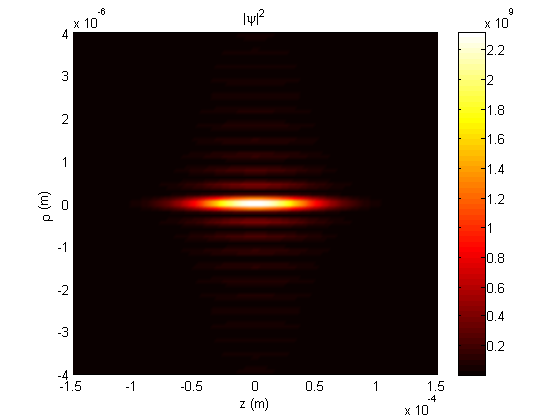
\includegraphics[scale=0.3]{figgau1c.png}}
\centering
\subfigure[]{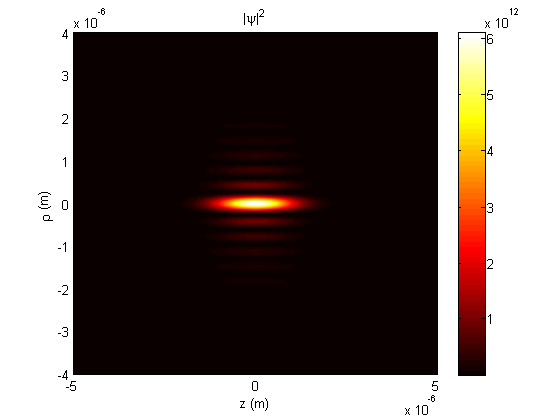
\includegraphics[scale=0.3]{figgau2c.png}}\\
\caption{(a)-(b) Gr\'aficos do espectro gaussiano n\~ao paraxial concentrado e n\~ao concentrado respectivamente. Os tra\c{c}os em vermelhos representam o espectro dado pela eq. (\ref{ga1}). Os tra\c{c}os em cor preta representam a representa\c{c}\~ao de (\ref{ga1}) atrav\'es da s\'erie de Fourier dada por (\ref{eqA19}). O n\'umero de termos de coeficientes de Fourier, para os  gr\'aficos foi de 801. (c)-(d) Padr\~oes de intensidade 3D, solu\c{c}\~oes exatas da equa\c{c}\~ao de onda dos feixes n\~ao paraxiais. (e)-(f) Proje\c{c}\~ao ortogonal da intensidade do feixe quadrado no plano $(\rho,z)$.}
\label{fig3}
\end{figure}
%*******************************************************************************
%*******************************************************************************
Do mesmo jeito dos itens anteriores foram analisados dois tipos de espectros n\~ao paraxiais.\\
O primeiro, um espectro $S(k_z)$ concentrado ao redor de $\bar{k}_z = 0,4\omega /c=3,97.10^6 m^{-1}$, com o desvio padr\~ao $1,99.10^{4}m^{-1}$ ($a=5,0.10^5/K^2$) e com $\Delta k_z/\bar{k}_z=0,005$. O gr\'afico do espectro (\ref{ga1}), no primeiro caso, \'e mostrado na Figura \ref{fig3}(a) em cor vermelha, sendo a sua representa\c{c}\~ao atrav\'es da s\'erie de Fourier (\ref{eqA18}) e mostrada em cor preta. O n\'umero total de coeficientes de Fourier usado foi de $801$, ou seja $N=800$.\\
O segundo espectro foi para uma largura de banda maior que a primeira $9,93.10^{5}m^{-1}$ ($a=200/K^2$) e com $\Delta k_z/\bar{k}_z=0,250$. O gr\'afico do espectro (\ref{ga1}) desse segundo caso \'e mostrado na Figura \ref{fig3}(b) em cor vermelha, sendo a sua representa\c{c}\~ao atrav\'es da s\'erie de Fourier (\ref{eqA18}) \'e mostrada em cor preta. O n\'umero total de coeficientes de Fourier usado para este \'ultimo espectro foi de $801$, ou seja $N=400$.\\
Na Figura \ref{fig3}(c)-(d) s\~ao apresentados os padr\~oes de intensidade em 3D. A Figura \ref{fig3}(c) corresponde ao espectro n\~ao paraxial concentrado obtido da Figura \ref{fig3}(a) e a Figura \ref{fig3}(d) corresponde a um espectro n\~ao paraxial n\~ao concentrado, obtido da Figura \ref{fig3}(b). Pode-se observar que quanto mais estreito \'e o espectro, maior ser\'a a profundidade de campo do feixe resultante.\\
Na Figura \ref{fig3}(e)-(f) s\~ao apresentadas as proje\c{c}\~oes ortogonais das intensidades dos feixes no plano $(\rho,z)$.  Os feixes obtidos prov\^em de espetros n\~ao paraxiais e s\~ao solu\c{c}\~oes anal\'iticas exatas da equa\c{c}\~ao de onda.\\
O espectro maior concentrado $1,99.10^{4}m^{-1}$ produz um feixe n\~ao paraxial com alcance de $1,0.10^{-4}$m (Figura $\ref{fig3}$(e)). Para um espectro menos concentrado $9,93.10^{5}m^{-1}$, o alcance do feixe n\~ao paraxial \'e de $2,0.10^{-6}$m (Figura $\ref{fig3}$(f)). Portanto, o feixe com espectro mais concentrado (Figura \ref{fig3}(a)), menor largura de banda, possui uma profundidade maior em rela\c{c}\~ao ao feixe menos concentrado (Figura \ref{fig3}(b)). Se fizemos  a largura de nossa gaussiana tender a zero, teremos como resultado um feixe de bessel, que possui concentra\c{c}\~ao do campo transversal e profundidade de campo infinita, portanto fluxo de pot\^encia infinito .  
%**************************************************************************************************************************
\section{Feixes Escalares puramente propagantes sem simetria azimutal}
Outro analise interessante \'e a obten\c{c}\~ao de de feixes n\~ao paraxiais sem simetria azimutal como solu\c{c}\~oes anal\'iticas exatas da equa\c{c}\~ao de onda. Feixes sem simetria azimutal podem ser constru\'idos como superposi\c{c}\~oes de fun\c{c}\~oes de Bessel de $\nu-$ordem, onde $\nu$ \'e um inteiro positivo. Do mesmo jeito que na obten\c{c}\~ao de feixes escalares n\~ao  paraxiais, os feixes sem simetria azimutal s\~ao complicados de obter devido \`a complexidade da integral neste caso, a integral em (\ref{eq11}). A seguir usaremos o mesmo m\'etodo matem\'atico usado anteriormente na obten\c{c}\~ao de feixes n\~ao paraxiais para solucionar (\ref{eq11}) e, portanto, fornecer solu\c{c}\~oes anal\'iticas exatas descrevendo feixes n\~ao paraxiais (e tamb\'em paraxiais) sem simetria azimutal puramente propagantes.\\
Partimos do feixe com simetria azimutal ($\psi(\rho,z,t)$) dado em (\ref{eqA20}), com espectro exponencial ($S(k_z)$) dado em (\ref{e1}). Usando (\ref{eq6}) obtemos um novo feixe sim simetria azimutal ($\psi_{1}(\rho,\phi,z,t)$) o qual \'e uma solu\c{c}\~ao exata da equa\c{c}\~ao de onda:
\begin{eqnarray}\label{eqs1}
\psi_{1}(\rho,\phi,z,t) &=& \frac{\partial\psi }{\partial \rho}\exp[{\rm i}\phi]\nonumber\\
\psi_{1}(\rho,\phi,z,t) &=&  \exp[-{\rm i}\omega t]\exp[{\rm i}\phi]\left( \frac{w^2}{c^2}\right)\sum\limits_{n=-\infty}^{\infty}R_n \rho  \left(\frac{\cos [h]}{h^2}-\frac{\sin [h]}{h^3}\right)
\end{eqnarray}
onde 
\begin{equation}\label{eqs2}
  R_n=\frac{1}{K}\int_{-\omega/c}^{\omega/c} S(k_z)\exp[-{\rm i}\frac{2\pi}{K}n k_z]dk_z
\end{equation}
\begin{equation}\label{eqs3}
h = \sqrt{\frac{\omega^2}{c^2}\rho^2+(z\frac{\omega}{c}+\pi n)^2}
\end{equation}
%*******************************************************************************
%*******************************************************************************
\begin{figure}[h]
\centering
\subfigure[]{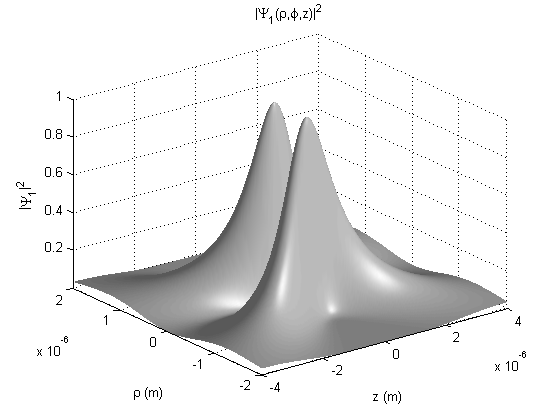
\includegraphics[scale=0.35]{figexSS1a.png}}
\centering
\subfigure[]{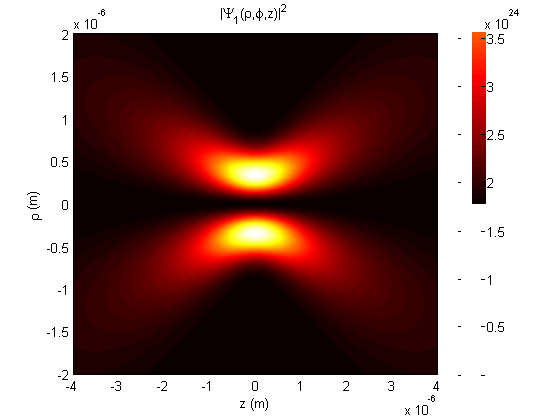
\includegraphics[scale=0.35]{figexSS1b.png}}
\centering
\subfigure[]{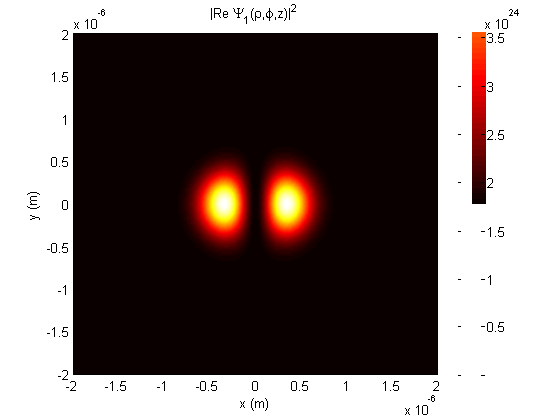
\includegraphics[scale=0.35]{figexSS1c.png}}
\caption{(a) Padr\~ao de intensidade 3D, solu\c{c}\~oes exatas da equa\c{c}\~ao de onda dos feixes n\~ao paraxiais sem simetria azimutal do espectro exponencial (\ref{e1}) para $\nu=1$. (b) Proje\c{c}\~ao ortogonal da intensidade do feixe quadrado no plano $(\rho,z)$. (c) Proje\c{c}\~ao ortogonal da parte real do feixe exponencial no plano $(x,y)$ para $z=0$.}
\label{fig4}
\end{figure}
%*******************************************************************************
%*******************************************************************************
Reparamos que a solu\c{c}\~ao exata (\ref{eqs1}) corresponde \`a superposi\c{c}\~ao dada em (\ref{eq11}), com $S^{'}(k_z)=S(k_z)(-k_{\rho})$, onde $S(k_z)$ esta dado por (\ref{e1}).\\
Foi analisado o espectro exponencial do tipo n\~ao paraxial ($S(k_z)$), com uma largura de banda $\Delta k_z = a = 100/K = 5,01.10^6 m^{-1}$. O gr\'afico do espectro (\ref{e1}) desse caso \'e mostrado na Figura \ref{fig1}(b) em cor vermelha, sendo a sua representa\c{c}\~ao atrav\'es da serie de Fourier (\ref{eqA18}) e mostrada em cor preta. O n\'umero total de coeficientes de Fourier usado foi de $801$, ou seja $N=400$.\\
Na figura \ref{fig4}(a) \'e apresentado o padr\~ao de intensidade normalizados em 3D. Notar que a Figura \ref{fig4}(a) corresponde ao espectro n\~ao paraxial $S^{'}(k_z)=S(k_z)(-k_{\rho})$, onde $S(k_z)$ \'e obtido da Figura \ref{fig1}(b). O feixe obtido prov\^e do espectro n\~ao paraxial e \'e solu\c{c}\~ao anal\'itica exata da equa\c{c}\~ao de onda. Podemos observar que o feixe produzido \'e propagante e n\~ao possui simetria azimutal ($\nu=1$).\\
Na Figura \ref{fig4}(b) \'e apresentada a proje\c{c}\~ao ortogonal da intensidade do feixe \ref{fig4}(a) no plano $(\rho,z)$ e na Figura \ref{fig4}(c) \'e apresentada a proje\c{c}\~ao ortogonal do quadrado da parte real do feixe \ref{fig4}(a) no plano $(x,y)$, com $z=0$. 
%*************************************************************************************************************************
